\documentclass[10pt]{article}

\usepackage{lipsum}
\usepackage{graphicx}
\usepackage{amsmath}
\usepackage{hyperref}

\usepackage[section]{placeins}

\usepackage{etoolbox}
\usepackage[onehalfspacing]{setspace}
\AtBeginEnvironment{figure}{\singlespacing}
\AtBeginEnvironment{table}{\singlespacing}

\usepackage{caption}
\DeclareCaptionFont{8pt}{\fontsize{8pt}{9pt}\selectfont}
\captionsetup{font={8pt}}


\usepackage[
	backend=biber,
    style=authoryear,
	url=false,
    %sorting=ynt,
    bibwarn=true,
    bibencoding=utf8,
    sortlocale=de_DE,
    maxbibnames=99,
    maxcitenames=1]{biblatex}
\renewbibmacro{in:}{}
    
\DefineBibliographyStrings{english}{
   andothers = {{et\,al\adddot}},}
   
\addbibresource{../../../bib/thesis.bib}

\AtBeginEnvironment{figure}{\singlespacing}
\AtBeginEnvironment{table}{\singlespacing}


\begin{document}


\begin{titlepage}
	\centering
	{\scshape\LARGE Ludwig-Maximilians-Universität München \par}
	{\scshape\large Faculty of Biology, Computational Neuroscience \par}
	\vspace{0.5cm}
	\includegraphics[width=0.4\textwidth]{../logo/siegel_black.pdf}\par
	\includegraphics[width=0.7\textwidth]{../logo/GSN-Logo_ab35mmBreite_RGB.jpg}\par
	\vspace{0.7cm}
	{\scshape\LARGE Master's Thesis \par}
	\vspace{0.05cm}
	\vspace{0.05cm}
	{\huge\bfseries Computational Simulation of Time Perception \par}
	\vspace{1.4cm}
	{\Large Katharina \textsc{M Bracher} \par}
	%{Student ID: 11754625 \par}
	\vspace{0.5cm}
	{\large Supervision: Dr. Kay \textsc{Thurley} \par}
	{\large Prof. Dr. Andreas \textsc{Herz} \par}
\end{titlepage}


\normalsize
\tableofcontents
%\the\textwidth 
%\makeatletter\f@size
% 345 pt = 4.79167 in -> figures 4.75 in 
% text 10 pt, fig caption 8 pt
% in drawio 10 pt -> 13.3; 8 pt -> 10.66 
\pagebreak


\section{Behavioral Effects in Magnitude Estimation}
Magnitude estimation is subject to noise that arises from external sources i.e. the statistics of the environment and internal sources i.e. neural representation of the input and the behavior.
Across sensory modalities, characteristic behavioral effects are identified (\cite{Petzschner2015}).
The most prominent observation is a regression to the mean of the stimulus range,  i.e. small stimuli are overestimated whereas large stimuli are underestimated (\textit{regression effect}). 
This effect intensifies for ranges with larger stimuli (\textit{range effect}).
For larger stimuli the standard deviation of estimates increases monotonically (\textit{scalar variability}). 
Finally, the recent history of stimuli presentations influences the current stimuli estimation (\textit{sequential effects}).
All effects mentioned above are displayed in Fig. \ref{fig:behavioraleffects}. 

Modality-independence of these effects suggests the existence of a common underlying principle or processing mechanisms, that would explain e.g. an optimal strategy for unreliable judgments due to noise (in stimuli and estimates).

\begin{figure}[ht]
	\centering
	\includegraphics[width=\textwidth]{figures/behavioural_effects_petzschner.pdf}
	\caption{\textbf{Behavioral effects.} 
	\textit{Regression effect}: in a range of stimuli large stimuli are underestimated, and small stimuli are overestimated which results in a regression to the mean of the range.
	\textit{Range effect}: the regression to the mean gets more pronounced for ranges that comprise larger stimuli. 
	\textit{Scalar variability}: the standard deviation of the reproduced magnitude grows linearly with larger rages. 
	\textit{Sequential effects}: the history presented stimuli (e.g. ascending or descending order) has an influence on the reproduced magnitude. 
	Adapted from \cite{Petzschner2015}.}
	\label{fig:behavioraleffects}
\end{figure}

During time perception and time reproduction experiments, neural activity displays characteristic trajectories in a low-dimensional space (\cite{Wang2018}, \cite{Henke2021}, \cite{Meirhaeghe2021}). 
The neural trajectories are consistently influenced by prior beliefs. 
Flexible motor timing can be achieved by controlling the speed of neural dynamics (\cite{Sohn2019}, \cite{Wang2018}). 
Further, it has been found that neural activity in anticipation of a delayed response reaches a fixed threshold with a rate inversely proportional to delay period (\cite{Murakami2014}, \cite{Mita2009}).
\cite{Wang2018} proposed a potential neural mechanism for speed control. Based on that mechanism \cite{Egger2020} developed an extended circuit model for sensorimotor timing.

\section{Model Description}
\subsection{Basic Circuit}
Flexible speed control can be achieved by a simple model consisting of three units, $u, v, y$ that represent population activity. 
The dynamics of $u, v$, and $y$ are defined as follows:
\begin{equation} \label{circuit}
	\begin{split}
	\tau\frac{\text{d}u}{\text{d}t} & = -u + \theta(W_{uI}I - W_{uv}v + \eta_u) \;, \\
	\tau\frac{\text{d}v}{\text{d}t} & = -v + \theta(W_{vI}I - W_{vu}v + \eta_v) \;, \\
	\tau\frac{\text{d}y}{\text{d}t} & = -y + W_{yu}u - W_{yv}v + \eta_y \;.
	\end{split}
\end{equation}
Two units, $u$ and $v$, receive a tonic symmetric input $I$ ($W_{uI}=W_{vI}=6$) and are mutually inhibiting each other ($W_{uv}=W_{vu}=6$). 
The inputs to $u$ and $v$ are governed by a sigmoidal activation function $\theta(x) = \frac{1}{1+exp(-x)}$.
The output unit $y$ receives excitatory input from $u$ and inhibitory input from $v$ ($W_{yu}=W_{yv}=1$) which results in a ramp-like activity of $y$.
All three units have a time constant $\tau = 100$ ms. 
Stochastic synaptic inputs are modeled as independent white noise $\eta_u, \eta_v, \eta_y$ with standard deviation $\sigma$.
Initial conditions of $u, v$ and $y$ have been optimized for in \cite{Egger2020} and are set to $u_0=0.7 , v_0=0.2 , y_0=0.5$ (Fig. \ref{fig:circuit}a)

Depending on the input $I$, the system shows different dynamics. For low levels of $I$ (0$<$I$<$0.5) the system has three fixed points (two stable, one unstable at $u=v$) and $y$ ramps up faster the higher input $I$. 
For intermediate values of $I$ (0.5$<$I$<$1) the system still shows three fixed points of the same sort as in the low input regime (Fig. \ref{fig:circuit}b)but $y$ ramps up with a slope that is inversely proportional to the input $I$ ($y$ ramps up slower the higher input $I$, see Fig. \ref{fig:circuit}c). 
For high $I$ (1$<$I) the system has one stable fixed point (at $u=v$) and $y$ ramps down faster for higher $I$.
Thus, the speed at which the output $y$ evolves can be controlled by the input $I$ (Fig. \ref{fig:circuit}d) and determines the time interval after which $y$ reaches a fixed threshold $y_{\text{th}}$. 
In interval reproduction experiments, reaching a threshold $y_{\text{th}}$ can be understood as movement initiation time which can be controlled for by adjusting $I$.
In this report, the intermediate input regime is explored: higher inputs result in a shallower slope of $y$, such that the threshold $y_{\text{th}}$ is reached after a longer time interval.

%%%%%%%%%%%%%%%%%%%%%%%%%%%%%%%%%%%%%%%%%%%%%%%%%%%%%%%%%%%%%%%%%%%% nullcline
\begin{figure}[ht]
	\centering
	\includegraphics{figures/defCircuit_nullcl.pdf}
	\caption{\textbf{Basic circuit and input regimes.} 
	\textbf{(a)} $u$ and $v$ share a common input $I$. The input is governed by weights $W_{uI}$ and $W_{vI}$. The two units have reciprocal inhibitory connections with weights $W_{uv}$ and $W_{vu}$ that determine the inhibitory strength. Both project to the output unit $y$ with an excitatory connection from $u$ and an inhibitory connection from $v$. Excitatory and inhibitory connections are shown by filled and open arrows, respectively. 
	\textbf{(b)} The control of the speed in $y$ can be analyzed in the phase plane of $u$ and $v$. The $u$ (dashed) and $v$ nullcline (solid) is shifted when the input is increased from $I=0.65$ (black) to $I=0.75$ (gray). In the intermediate regime the systems shows two stable and one unstable fixed point. The red cross indicates the initial conditions for the dynamics in (c). Depending on $I$, with the same initial conditions, the system evolves faster or slower to the stable fixed point. 
	\textbf{(c)} Dynamics of $y$ for intermediate regime with input $I=0.75$ in gray and $I=0.65$ black. There is an inverse relation of input strength and slope. With higher input, the threshold at 0.7 (dashed line) is reached after a longer time interval. 
	\textbf{(d)} Dynamics of $u, v, y$ for inputs from $0.1\leq I \leq 1.5$ are shown. Initial conditions are set to $u_0=0.7 , v_0=0.2 , y_0=0.5$. With these initial conditions and values of $I>=0.5$, the relation of steady state activity of $y$ (and slope to reach the steady state) is inverse to $I$ (intermediate and high $I$ regime). For values $I<=1$ the activity of $y$ ramps down (yellow corresponds to $I=1$). For $I<0.5$ the steady state (slope) is smaller the smaller $I$ (low $I$ regime, dark blue).}
\label{fig:circuit}
\end{figure}

\subsection{Update Mechanism and Experiment Procedure}
Basic interval reproduction experiments can be designed with only two epochs: a measurement epoch that has the duration of the stimulus interval and a reproduction epoch that starts immediately after the measurement epoch (Fig. \ref{fig:epochs}b). 
The basic circuit described above is modified to perform interval reproduction (see Figure \ref{fig:epochs}a for schematic of modified circuit).
The relation of input $I$ with the slope of the ramping activity of $y$ is used in combination with a fixed threshold $y_{\text{th}}$.
By adding an update mechanism that flexibly adjusts $I$, the threshold crossing of $y$ can be delayed or moved to earlier times.
This way, measuring and reproducing an interval is done predictively, by adjusting the slope of the ramp such that the output reaches the threshold after the intended time.
%In other scenarios, time could be encoded by the level a ramp reaches with a fixed slope.
In the model the measurement epoch is fixed to the stimulus interval $t_s$, and the reproduction epoch ends, when $y$ reaches the fixed threshold $y_{\text{th}}$ from below. 
The time from the end of the measurement epoch until the threshold-crossing of $y$ yields the reproduced time interval $t_r$ that is aimed to equal the stimulus interval $t_s$ (Fig. \ref{fig:epochs}c).

\begin{figure}
	\centering
	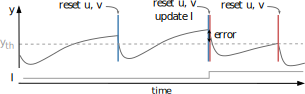
\includegraphics{figures/epochs.pdf}
	\caption{\textbf{Extended circuit for experiment simulation.} 
	\textbf{(a)} The circuits for measurement, reproduction and delay epoch are displayed. All circuits comprise the same basic structure with different additional elements that are unique for the epoch. Initial values of $u, v, y$ and $I$ are fed into the delay circuit for the duration of the initial interval. $u$ and $v$ are reset with a transient input $I_r$ before end values of $u, v, y$ and $I$ are transferred to the measurement circuit as new initial conditions. After the duration of the stimulus interval the difference between $y$ and the threshold $y_{\text{th}}$ is used with the memory parameter $K$ to update $I$ together with another reset of $u$ and $v$. The values are transferred with all other variables to the reproduction circuit. The reproduction epoch ends when $y$ reaches the threshold $y_{\text{th}}$ from below. Before the presentation of another stimulus interval, there is again a delay period with no update of $I$. The reset mechanism enables the model to simulate an arbitrary number of stimulus intervals. Adapted from \cite{Egger2020}.
	\textbf{(b)} Interval reproduction experiment with stimulus interval $t_s$ (blue) and reproduction $t_r$ (red).
	\textbf{(c)} Schematic of one trial. After a delay epoch $u$ and $v$ are reset. The measurement epoch lasts for the duration of the stimulus interval $t_s$. $y$ should reach the threshold $y_{\text{th}}$ (dashed line) at exactly the time the stimulus interval ends. The threshold was crossed well before the end of the interval and at the end of the measurement epoch, the error in $y_m$ to the threshold $y_{\text{th}}$ is used to update $I$. To reach the threshold at a later time, $I$ is increased, which reduces the slope of $y$ in the reproduction epoch. After the reset of $u$ and $y$ and the update of $I$ the reproduction ends when $y$ reaches the threshold. The time after the reset and update until the threshold crossing denotes the reproduced interval $t_r$.}
\label{fig:epochs}
\end{figure}

The following update mechanism of $I$ is based on the intermediate input regime, that shows an inverse relation of $I$ to the slope of $y$ (Fig. \ref{fig:circuit}b).
The error signal is determined at the end of the measurement epoch and is composed of the difference of $y$ to the threshold $y_{\text{th}}$.
If the threshold $y_{\text{th}}$ is not reached during the measurement epoch, the slope has to be adjusted, such that $y$ ramps up faster to reach the threshold at exactly the time of the stimulus interval. For a steeper slope, $I$ is reduced.
If $y$ crossed the threshold before the measurement epoch ends, so is above $y_{\text{th}}$ by the end of the stimulus interval, the slope needs to be reduced in order to reach the threshold at a later time in the reproduction. For a shallower slope, $I$ is increased (Fig. \ref{fig:epochs}c).
$I$ is adjusted according to the error $(y-y_{\text{th}})$, weighted by a memory parameter $K$ right at the end of the measurement epoch
\begin{equation} \label{Iupdate}
	\begin{split}
	\tau\frac{\text{d}I}{\text{d}t} & = sK(y-y_{\text{th}}) \;.
	\end{split}
\end{equation}
The update of $I$ is only active for a pulse between the measurement and reproduction epoch ($s=1$) and inactive for all other times ($s=0$).
Further, $u$ and $v$ receive a transient input pulse $I_r$ to reset the dynamics for the subsequent epoch (Fig. \ref{fig:epochs}c)
\begin{equation} \label{experimentcircuit}
	\begin{split}
	\tau\frac{\text{d}u}{\text{d}t} & = -u + \theta(W_{uI}I - W_{uv}v + \eta_u - I_r) \;,\\
	\tau\frac{\text{d}v}{\text{d}t} & = -v + \theta(W_{vI}I - W_{vu}v + \eta_v + I_r) \;.\\
	\end{split}
\end{equation}
Resetting the dynamics after the reproduction epoch enables the model to simulate an arbitrary number of stimulus intervals. 
Before a new stimulus presentation there is a delay period: In the beginning of an experiment with a sequence of stimuli there is an initial interval with the initial values of $u, v, y$ and an initial input $I_0$ (Fig. \ref{fig:epochs}c). 
This additional interval in the beginning of the experiment allows the model to get closer to steady-state before the stimulus presentation starts. 
Reproductions that do not reach the threshold in a certain time span  or too early are classified as timeout trial.
%sup

To simulate variability in the reproductions as it is found in real data, noise is added to $u, v$ and $y$ in the implementation. In data a monotonic increase of the standard deviation of reproductions is found (\textit{scalar variability}). 
If noise levels in the model are too high ($\sigma>0.2$) the standard deviation of reproductions is not growing monotonically with $\sigma$ (\cite{Egger2020}).
For all simulations $\sigma$ was set to 0.02, which results in realistic coefficient of variation of 0.1 (Supplementary Fig. \ref{sup:CV}b, c).
%todo: cite plausible CV
In Figure \ref{fig:experiment}a five example trials and the activity of $u, v, y$ and $I$ are depicted. 
In the full simulation, 500 stimuli randomly chosen from a stimulus distribution were presented. The uniform distribution of time intervals is denoted as stimulus range. 
The stimulus range consisted of seven stimuli ranging from 400-700 ms (\ref{fig:experiment}b).

The experiment simulation results in a distribution of reproduced time intervals for each stimulus and a distribution of inputs that drive the activity of $y$ in the reproduction (Fig. \ref{fig:experiment}c).
Taking the mean over the distribution of reproduced time intervals for each stimulus allows for the investigation of effects in the behavioral results (Fig. \ref{fig:experiment}d). 

\begin{figure}[ht]
	\centering
	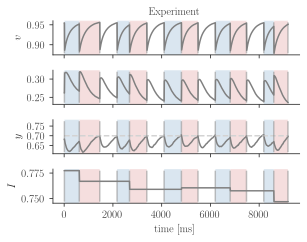
\includegraphics{figures/trial.pdf}
	\caption{\textbf{Experiment description.} 
	\textbf{(a)} The dynamics of $u, v, y $ and $I$ are displayed over time for five consecutive example trials (650, 500, 600, 700, 450 ms) of an experiment simulation with 500 trials. Stimulus presentation and reproduction epochs are highlighted in blue and red, respectively. Before new stimuli presentations, there is a 700 ms delay period (white). Initial values for the experiment simulation are set to $u_0=0.7 , v_0=0.2 , y_0=0.5, I_0=0.8$. The added noise is set to $\sigma=0.02$ and the memory parameter to $K=5$. The threshold is set to $y_{\text{th}}=0.7$ (dashed line). Reproduced times are 690, 540, 550, 650, 490 ms.
	\textbf{(b)} For the experiment simulation time intervals were randomly drawn from a discrete, uniform stimulus distribution. The range of time intervals contained stimuli from 400 to 700 ms with steps of 50 ms.
	\textbf{(c)} The measurement (upper) and reproduction (middle) epoch of $y$ and input for reproduction (lower) are shown for the full experiment sorted according to stimulus interval. Shown are trials for stimuli of 400, 550 and 700 ms (depicted above).
	\textbf{(d)} Mean reproduction and standard deviation (black) across trials for each stimulus interval of the experiment stimulation shown (c). If the mean lies on the identity line (dashed line), mean reproduction time corresponds to the stimulus interval. Red dots show the reproductions of the example trials shown in (a). 
	}
\label{fig:experiment}
\end{figure}

\section{Memory Parameter in Accordance with Error Minimization}
We asked whether the observed behavioral effects in real data (Fig. \ref{fig:behavioraleffects}) can be reproduced by experiment simulations with the circuit model that is based on the scaling phenomenon found in brain data. 
A crucial value to optimize for is the memory parameter $K$, which defines the weight with which the input is adjusted to balance the mismatch between the predicted interval and the stimulus duration.
Another parameter that is necessary to tune is the time constant $\tau$, which influences how fast $y$ evolves in response to the input. Hence, $\tau$ can be interpreted as a biophysical parameter of the model.
In contrast to \cite{Egger2019}, other parameters like initial values, in particular $I_0$ don't have to be optimized in this simulation. In the experiment simulation only the first one to two trials are influenced by the initial values.
%weights 
%noise adjusted to plausible CV in results
The threshold was set to 0.7, but smaller and larger thresholds were tested as well.

 
\subsection{Behaviorally Plausible Slopes}
Biological plausible slopes in behavioral results lie around 0.83 for the short and 0.73 for the long range (\cite{Thurley2018}, \cite{Jazayeri2010}). 
In wide parameter regimes, the reproductions show a regression to the mean. For fixed $\tau$, the slope increased with increasing $K$, since more weight is put on the current update, in other words relying less on the prior. 
Choosing suitable values for $K$, the model also produced plausible slopes for various time constants (Fig. \ref{fig:parameter}a), where $K$ has to be adjusted according to the stimulus range and time constant. 
$K$ is set to smaller values for the long range, putting less weight on the update compared to the short range, to produce plausible slopes.

\subsection{Optimization of Parameters}
Can behavioral effects also be achieved by adjusting $K$ in accordance with error minimization?
To find optimal values for $K$ mean squared error was minimized, defined as the sum of the squared bias and variance of the mean reproductions (Supplementary Eq. \ref{MSE}).
For evaluating effects in behavior, two stimulus ranges were used in simulations, denoted as short and long range with stimuli ranging from 400-700 ms and 700-1000 ms, respectively. Both ranges contained a 700 ms stimulus interval.

For larger time constants $\tau$ the optimal $K$ increased. For all time constants optimal values of $K$ were smaller for the long range compared to the short range, as already found for values of $K$ that result in plausible slopes.
The corresponding time constant $\tau$ for the overall minimum of the MSE differed between the two stimulus ranges. For the short stimulus range, $\tau = 120$ ms, $K = 11$ yielded the overall minimum, for the long range the parameter pair was $\tau = 200$ ms, $K = 20$. 
For the experiment simulation we had to find a common $\tau$ for the short and long range. Consequently, a time constant between the optimums was chosen, based on the overlap with biological plausible slopes. Only with a time constant of 130 ms, optimal $K$ coincided with biological plausible slopes in both ranges. 
Corresponding optimal values for $K$ with a time constant of 130 ms were 13 for the short and 10 for the long range (Fig. \ref{fig:parameter}b, Supplementary Fig. \ref{sup:othererror}a, b).
Behavioral results show a regression to the mean with a stronger regression for the long range (range effect) (Fig. \ref{fig:parameter}c). For dynamics of $y$ over the whole experiment see Supplementary Fig. \ref{sup:experiment}.
Adjusting $K$ in accordance with error minimization, leads to putting more weight on the prior experience for longer stimuli, which naturally entail more uncertainty, and is thus biological plausible.
Yet, the slope for the small ranges lies below the slopes found in data. 
The standard variation of reproductions increases linearly (scalar variability), the mean coefficient of variation (CV) for the short range is 0.09, for the long range 0.11 (Fig. \ref{fig:parameter}d).
Furthermore, a general underestimation for the large range is observed for all time constants (Supplementary Fig. \ref{sup:othererror}e). This is probably the case due to high variance that pushes $K$ to lower values.
When optimizing for the squared bias or variance only, no range effect is observed and the relation of smaller $K$ for longer stimuli, so putting more weight on the prior is not apparent for both options (Supplementary Fig. \ref{sup:othererror}c, d).  
%supp

\begin{figure}[ht]
	\centering
	\includegraphics{figures/interIparams.pdf}
	\caption{\textbf{Behavioral effects and parameter optimization.} 
	\textbf{(a)} Simulations with 500 trials for each pair of memory parameter $K$ and time constant $\tau$ at noise level $\sigma = 0.02$. Simulations were performed with stimuli chosen from the short (left) or long range (right). Color scale represents the slope of the linear fit between stimuli and reproductions. A slope of 1 on the identity line corresponds to perfect reproduction of the stimuli. Behaviorally plausible slopes are encircled in blue and lie around 0.83 for the short and 0.73 for the long range. Empty spaces show simulations, that exceeded the number of timeout trials and where thus excluded from analysis.
	\textbf{(b)} Optimization of the weight given to the update, $K$, for different time constants $\tau$ at noise level $\sigma = 0.02$. Color scale represents the MSE for an experiment stimulation with 500 trials for each pair of $K$ and $\tau$. Stimuli were either chosen from the short (left) or the long stimulus range. The minimal error for each $\tau$ is encircled in black and minimal error across all $\tau$ is additionally crossed. Parameter combinations that result in behaviorally plausible slopes (a) are shaded in blue.
	\textbf{(c)} Mean reproductions for simulation with 500 trials for each stimulation with the short (black) and long (gray) stimulus range. The value of $K$ is optimized for a time constant of $\tau = 130$ ms. For the simulation with short stimulus range optimal $K$ was 13, with the long stimulus range optimal $K$ was 10. 
		Insert: For experiment simulations two stimuli ranges were used. The short range contained stimuli from 400 to 700 ms, the long range contained stimuli from 700 to 1000 ms.
	\textbf{(d)} Standard deviation of reproductions for each stimulus for the short and long range from the simulation in (c).
	}
\label{fig:parameter}
\end{figure}

\section{Comparison of Intermediate and High Input Regime}
Between the intermediate and high input regime are elementary differences concerning the fixed points and dynamics. Yet, simulations of time reproduction experiments are possible on both regimes. In the following the input regimes are compared and simulations and optimization are performed for the high input regime.

\subsection{Comparison of Dynamics}
Where in the intermediate input regime three fixed points emerge in the phase plane (2 stable and on unstable), the fixed points merge to one when in the high input regime. 
The single fixed point is situated in comparably high activity of $u$ and $v$(Supplementary Fig. \ref{sup:comparison}a, d). 
This influences the dynamics in $u$ and $v$ such, that $y$ ramps up in the high regime instead of down in the intermediate regime. 
The dynamic in $u$ and $v$ results in a steeper slope of $y$ for higher $I$ in the high input regime and is thus reversed compared to the intermediate input regime (Fig. \ref{regimes}). 

\begin{figure}[ht]
	\centering
	\includegraphics{figures/supp_regimes.pdf}
	\caption{\textbf{Comparison of dynamics in the intermediate and high input regime.} 
	\textbf{(a)} Evolution of $u, v$ and $y$ over time for different inputs from 0.5 to 0.95 in the intermediate input regime. Activity in $y$ shows a ramping-up activity. The activity of $y$ evolves to different steady states depending on the input. 
	\textbf{(b)} Gradient of $y$ over time for different inputs in the intermediate regime. Lower input results in higher gradient, where the gradient is maximal for the input 0.5.
	\textbf{(c)} Same as (a) for the high input regime with inputs from 1.01 to 1.5. Activity in $y$ shows a ramping-down activity, converging to 0 independent of input.
	\textbf{(d)} Same as (b) for high input regime. Higher input results in higher absolute gradient. 
	}
\label{regimes}
\end{figure}

\subsection{Experiment Simulation in the High Input Regime}
To simulate time reproduction experiments in the high input regime a few minor changes to the parameters have to be done. 
The threshold is set to a lower value but above 0 (e.g. 0.05 or 0.1) and initial $I$ is set to a value above 1 ($I_0 = 1.02$). The reset impulse after each epoch to $u$ and $v$ has to be stronger with a factor of 10 and with opposite sign to put the activity in $y$ to a higher level again.  

\begin{equation} \label{highI}
	\begin{split}
	\tau\frac{\text{d}u}{\text{d}t} & = -u + \theta(W_{uI}I - W_{uv}v + \eta_u + 10*I_r) \;,\\
	\tau\frac{\text{d}v}{\text{d}t} & = -v + \theta(W_{vI}I - W_{vu}v + \eta_v - 10*I_r) \;.\\
	\end{split}
\end{equation}

There is no need to change the update mechanism, even though the relation of the input $I$ and the slope is reversed. This is because $y$ ramps down and approaches the threshold from above and not from below, so that the relation of $y$ and $y_{\text{th}}$ is reversed and the update of $I$ is correct. 

The noise was set to the same value as in simulations in the intermediate regime ($\sigma$ = 0.02). The standard deviations increased linearly for a wide range of noise levels. For increasing $\sigma$ the standard deviation drops slightly and then plateaus for $\sigma$ larger than 0.1. For a $/sigma$ of 0.02, the CV took similar values as in the intermediate regime with 0.13 for the short and 0.12 for the long range (Supplementary Fig. \ref{sup:highI}a). 
An example of the experiment dynamics for four consecutive simuli is displayed in Fig. \ref{highI}a.

\subsection{Parameter Optimization in the High Input Regime}
Optimization was performed for the time constant $\tau$ and the memory parameter $K$ with the same stimulus ranges as in the intermediate regime. 
Also in the high input regime biologically plausible slopes were produced for most $\tau$. 
For all $\tau$ larger 40, optimal $K$ were smaller for the long range compared to the short range.
The MSE was minimal across all time constants for $\tau = 60$ for both the short and the long range with optimal $K$ at  4 and 2.5 for the short and the long range, respectively. The combination of optimal $\tau$ and $K$ resulted in a biologically plausible slope only in the long range, for the short range the slope was not steep enough. 
Behavioral results of experiment simulation with optimal parameters show a regression to the mean. For the long range a general underestimation of all stimuli is apparent. Also, standard deviations of the reproductions do not grow linearly especially for the long range (Supplementary Fig. \ref{sup:highI}b, c).
For dynamics of $y$ over the whole experiment see Supplementary Fig. \ref{sup:experiment_high}.

\begin{figure}[ht]
	\centering
	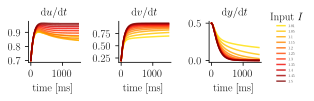
\includegraphics{figures/highI.pdf}
	\caption{\textbf{Experiment Simulation in the High Input Regime.} 
	\textbf{(a)} Activity of $u, v, y$ and $I$ for five example stimulus intervals of 650, 500, 600, 700, 450 ms. Stimulus presentation and reproduction epochs are highlighted in blue and red, respectively. The delay period between trials is shown in white. Initial values are set to $u_0=0.8 , v_0=0.6 , y_0=0.1, I_0=1.04$ and the threshold $y_{\text{th}}$ is set to 0.1. 
	\textbf{(b)} Mean reproductions for simulation with 500 trials for each stimulation with the short (black) and long (gray) stimulus range. The value of $K$ is optimized for a time constant of $\tau = 60$ ms. For the simulation with short
	stimulus range optimal $K$ was 4, with the long stimulus range optimal $K$ was 2.5.
	\textbf{(c)} Standard deviation of reproductions for each stimulus for the short and long range from the simulation in (b).
	}
\label{highI}
\end{figure}

\subsection{Comparison of Optimal Experiment Simulations}
To compare the experiment simulations of the intermediate and high input regime, results produced by the optimal parameter combinations were used with the dynamics displayed in Supplementary Fig. \ref{sup:experiment} for the intermediate and \ref{sup:experiment_high} for the high input regime.
The maximal and minimal input $I$ during the simulation with either the short or the long range were used in the phase plane to plot the nullclines of $u$ and $v$ furthest apart from each other (Supplementary Fig. \ref{sup:comparison}a, d).
For each stimulus the mean input $I$ during the experiment simulation shows an almost linear increase (or decrease) within a range. The increase (or decrease) is shallower for the long range due to the smaller optimal $K$ used in the simulation. 

%%%%%%%%%%%%%%%%%%%%%%%%%%%%%%%%%%%%%%%%%%%%%%%%%%%%%
\section{General Underestimation}
%motivate why interesting
In experiment simulations with optimal $K$, a general underestimation in the long stimulus range occurs (Fig. \ref{fig:parameter}c, Supplementary Fig. \ref{sup:othererror}a, b, \ref{sup:highI}e).
%todo ind point
The indifference point lies at....
What is the reason for the general underestimation of larger inputs? 
It is not uncommon, that stimuli in larger ranges are generally underestimated in magnitude estimation in behavioral data (\cite{Petzschner2012}).
%Todo: citation underestimation
The cause of however has not been investigated and could have many reasons ranging from decreasing attention to impatience. 
It needs to be investigated if the underestimation present in the model is caused by the model used in this experimental setting, or if it is a phenomenon that emerges due to optimality in parameter choices. %???????????????
Possible (hyper)parameter choices that might influence the behavior are the delay period between trials, the fixed threshold and the shared time constant. 
%Todo: what about the extremes? when does the model stop working
%Todo: add real behavioral plots -f4 drive

\subsection{Delay Period Influences Estimates}
Simulations were performed with a compromised time constant $\tau$ between the optimal $\tau*$ for the short and long range, respectively.
General underestimation in simulations with the long range can be counteracted by increasing the time constant towards the optimum of the long range. (Supplementary Fig. \ref{sup:othererror}b). This causes a general overestimation in the simulation with the short range with a shared time constant. 
Thus, the time constant $\tau$ contributes to the under- and overestimation of stimuli, when set to far from the range's optimum. But even at the optimum, simulations with the long range still show a slight general underestimation.
%inhibitorische population schiebt rate 
So there might be multiple causes for this problem.

Another observation in the behavioral results is, that the best reproductions in the short range were made for stimuli above 600 ms and for the long range for simuli below 800 ms. So stimuli between 600 and 800 ms were resulted better reproductions  across ranges. 
We simulated an experiment with a stimulus range that had stimuli between 550 and 850 ms (550, 600, 650, 700, 750, 800, 850 ms), with a mean of 700 ms. This corresponds to the length of the fixed delay period of all previous simulations. In Fig. \ref{fig:delay}a the behavioral results of a simulation with optimal $K*$ and $\tau*$ show regression to the mean with a slope of 0.82 and an indifference point of 657 ms.
A delay period of 700 ms corresponds to the maximum of the short range and the minimum of the long distribution. 
When setting the delay period at the maximum of the long range instead (1000 ms), a general overestimation of stimuli from the short range occurs with mean optimal $\tau$'s (Supplementary Fig. \ref{sup:delay}c).
This led to the assumption, that a delay period that is close to the range's mean over- or underestimation. 
A delay period that is relatively short compared to the stiumli in an experiment leads to wrong updates, since the dynamic in $y$ is not able to reach threshold level in the short time period with mean $I$. 
After a reset the subsequent measurement period is then starting from lower values in $y$. 
Setting the delay period equal to the mean of the range results in better reproductions 
(Supplementary Fig. \ref{sup:delay}a, b).

Shifting the threshold to higher or lower values of $y$ does not resolve under- or overestimation. However, the threshold has to be set in an appropriate scope to avoid exceeding timeouts. 

%todo what about high I regime?
%todo underestimation extra long: grenzen des Models, remapping zwischen ms und s, einem festen 
% K small tau large

\subsection{Adjusted Experiment Simulation}
The previous analysis showed, that there are two main problems that caused distorted reproductions. 
First, a compromised, shared time constant between experiments with different ranges skews the reproductions.
Since the time constant in the model can be interpreted as a rate time constant, it is justifiable to change it between experiment. 
This would correspond to an adjusted rate in the population to an experiment setting.
Second, it is the application of the model in the described experimental setting. The delay period between trials is a hyperparameter of the experiment design that should not influence reproductions.
Thus, the model needs to be adjusted to take into account the experimental design. 
% delay=mean of range
Setting the time of the delay epoch to the mean of the range that is used in the experiment simulation doesn't make sense from a design point of view. It should be possible to choose the delay time between trials arbitrarily and independent of the stimulus range. 
% long delay + separate tau
Similarly, the delay period can be set to a time that is sufficiently long, such that the system evolves to a steady state. With the addition of optimized $\tau$ for stimulus ranges independently, distorted reproductions can be avoided. Again. this would mean no independent choice of the delay period.
% no delay
Another possibility that solves the problem arising from the length of the delay epoch, is discarding the delay in the experiment design (Fig. \ref{fig:delay}b).
This solves the problem, because the reproduction period always ends when the threshold is met, thus the subsequent reset and measurement period begin at the same values in $y$.  
This does not necessarily mean, that the experimental design is restricted. When simulating experiments that include a delay period between trial or even between measurement and reproduction, it can be assumed, that information is hold in the system until the next epoch starts. 
It has been shown in neural networks, that information about time can be hold in state space over a delay period (\cite{Bi2020}).
This can be combined with independent, optimal $\tau$ for each range as discussed above (Fig. \ref{fig:delay}c).
Simulations in section \ref{externalvar} are performed without delay period between trials.
% reset on fixed value
% learn I for delay
Solutions that incorporate a delay period in the simulation itself would need model adjustments,
Either the reset is changed from an impulse to a fixed reset value or the input $I$ during the delay epoch is not adopted from the previous trial but updated separately based on an error in order to always reach the threshold. 


\begin{figure}[ht]
	\centering
	\includegraphics{figures/delay.pdf}
	\caption{\textbf{Behavioral results with matched or no delay.} 
	\textbf{(a)} Behavioral results of an experiment simulation with the previously utilized delay of 700 ms. The stimulus range that was used to sample stimuli from has a mean equal to the delay of 700 ms. The time constant and update parameter were both optimized based on the MSE ($\tau$ = 170 ms, $K$ = 17.5). Other parameters like threshold and initial values were not changed. 
	\textbf{(b)} The delay period was set to 0 ms in simulations with the short and long range (black and gray, respectively). The time constant was set to 165 ms, which corresponds to the mean of the optimal $\tau$ for the short (130 ms) and long (200 ms) range. For $\tau$ = 165 ms, the update parameter $K$ was optimized (short range $K$ = 21, long range $K$ = 13). Note different axes of figures in (a) and (b).
	\textbf{(c)} Same as (b) but with independent, optimal time constant. For the short range $\tau*$ = 130, $K$ = 14 and for the long range $\tau*$ = 200, $K$ = 20.
	}
\label{fig:delay}
\end{figure}

\section{Influence of External Variability on Behavior} \label{externalvar}
Regression to the mean depends on the discrimination abilities of the individual subject. This is reflected by internal noise $\sigma$ in the model.
Additionally, variability of the environment influences the behavior, which is captured  by the statistics of stimuli over the course of an experiment. 
The statistics if stimuli can be summarized by the ratio of the mean and variance of the stimulus range: $\frac{\text{E(t)}}{\text{var(t)}}$.
When internal noise is fixed, the external variability can be modified independently. 
Since optimized $K$ reflects inversely the weight on the prior, the effect of external variability on the update parameter can be investigated by modifying the mean or the variance of stimuli. 

\subsection{Effects of Stimuli Statistics in Real Behavior}
With larger interval times, internal estimates get noisier and regression of reproductions gets stronger. This is well described by the \textit{range effect} across species (\cite{Cicchini2012} \cite{Sohn2019}, \cite{Henke2021}). 
Increasing the mean interval of stimuli, increases the external variability ratio
and as a result more weight should be put on the prior (stronger regression, $K$ decreases).
Besides the mean, also the variance of a stimulus distribution influence the reproduction of intervals.
Larger variance can be achieved by reducing the sampling frequency in a range or by expanding the span of a range, accommodating more distance time intervals. 
The effect of variance of stimuli on the behavior is not well investigated.
There are three conceivable possibilities. 
Reproductions could get better, hence regression weaker. This would mean putting more weight on the update ($K$ increases) instead of the prior. 
Intuitively, larger variance means that differences of time intervals get more apparent and discrimination becomes easier (e.g. stimuli are further apart or extremes are more distinct). 
This scenario is predicted by model that used noisy integrators linked by an adaptive reference in \cite{Thurley2016}.
On the other hand, a change in variance with fixed mean could have no effect on the behavior. Then only the mean would have an effect on the reproduction performance.
This seems to be the case in \cite{Petzschner2012}, where performance of the range with larger variance doesn't get better. 
Finally, reproductions could get worse with larger variance. This has been demonstrated in sound intensity by \cite{Teghtsoonian78}.
Most studies that include experimental data with stimuli ranges that differ in variance did not investigate the effect on regression. 

\begin{figure}[ht]
	\centering
	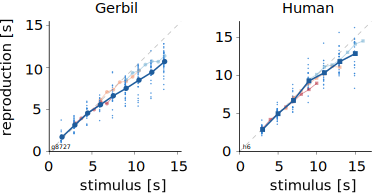
\includegraphics{figures/underestimation.pdf}
	\caption{\textbf{Effects of stimuli statistics in behavior of gerbils and humans.}
	Reproductions of stimuli that are several seconds long in four experiments with different ranges: short (red), mid (orange), long (light blue) and all (blue). Ranges differed slightly between experiments with gerbils and humans. 
	Large markers display the mean of trials.  Small dots show trials for the experiment with the all range.
	\textbf{(a)} Behavioral results of a gebril.
	\textbf{(b)} Behavioral results of a human.
	Figure courtesy of Kay Thurley and Josephine Henke.
	}
\label{fig:underestimation}
\end{figure}


\subsection{Optimality Predicts Regression Effect and Range Effect across Ranges.}
So far the short and the long range have been used in simulations. Both comprised seven stimuli that spanned 300 ms and had their mean at 550 and 850 ms, respectively. 
Additional ranges that differ in mean, span and sampling were created to test the behavioral predictions of the model based on the external variability of stimuli.  
Two ranges with same variance and span but with shifted means at 700 ms (mid range) and 1050 ms (extra-long range) were used for simulations. Based on the external variability ratio, $K$ should decrease with increasing mean of a range. 
Additionally, ranges with a mean equal to one of the ranges mentioned above, but higher variance were examined.
Including all stimuli from both the short and the long range, the all range has its mean equal to the mid range but a wider span (600 ms) and thus higher variance.
The short-few and all-few range span the short and the all range, respectively, but with an under sampled number of stimuli and thus in each case higher variance
(Fig. \ref{fig:new_ranges}a, Supplementary Fig. \ref{sup:ranges}c).

Experiment simulations were performed with a threshold of $y_{\text{th}}$ = 0.7 and $\sigma$ = 0.02. The time constant $\tau$  was set to 165 ms for all stimulus ranges, which corresponds to the mean of the optimal $\tau*$ of the short (130 ms) and long (200 ms) range. 
Optimal $\tau*$ for other ranges were the following: mid 170 ms, extra-long 230 ms, all 150 ms and short-few 120 ms. 
As expected, optimal $K$ for the mid range (16.71) was lower compared to the short range (21.33) but higher compared to the long range (13.10) due to the shifted mean 
(Kolmogorov–Smirnov two-sample test, n=20 for each distribution, p$<$0.01, Bonferroni correction for multiple testing, this also applies for all following comparisons if not denoted as not significant).
For the extra-long range (8.71), optimal $K$ was smaller than for the long range.
Across the four ranges optimal $K$ has an almost linear relationship with shifting mean.
Decreasing $K$ for increasing mean of ranges is captured by the model beyond the short and the long range (Fig. \ref{fig:new_ranges}b).
Corresponding slopes in the behavioral analysis all show slopes below zero. Thus, optimal $K$ is predicting the regression effect across multiple ranges (Supplementary Fig. \ref{sup:ranges}a). 
There is no significant difference in the slope of behavior in the short and the mid range, but otherwise significant decrease in the slope with increasing mean. The model therefore only predicts the range effect for large enough changes in the mean. 
The optimal time constant $\tau*$ of the mid range (170 ms) is closest to the shared time constant of 165 ms for all simulations
(Kolmogorov–Smirnov two-sample test, n=21 for each distribution, p$<$0.01, Bonferroni correction for multiple testing).
But even when the constraint on the time constant is relaxed and allowed to change between experiment simulations, the slope of behavioral results of simulations, which were performed with optimal $K$ and optimal $\tau*$, show no significant difference between the short and the mid range(Supplementary Fig. \ref{sup:ranges}b)
(Kolmogorov–Smirnov two-sample test, n=21 for each distribution, Bonferroni correction for multiple testing).

\subsection{Optimality Predicts No Influence of Variance on Behavior.}
How does optimal $K$ and the slope change when the mean is fixed, but variance is increased?
The increased variance has no influence on neither $K$ nor the slope (Fig. \ref{fig:new_ranges}b, c; Supplementary Fig. \ref{sup:ranges}a, b).
Higher variance in the ranges with fewer stimuli (short-few, all-few) shows no significant difference to their counterparts with higher stimulus sampling (short, all).
Also, a larger span of stimuli (all range) results in no significantly larger or smaller $K$ compared to a range with smaller span (mid range) 
(Kolmogorov–Smirnov two-sample test, n=21 for each distribution, Bonferroni correction for multiple testing).

The model predicts, that only the mean has an effect on the regression in reproduction performance. This is supported by data in \cite{Petzschner2012}, however more studies that investigate this particular phenomenon have to be performed to validate this prediction. 
The circuit model is making opposing predictions to the noisy integrator model by \cite{Thurley2016}.

\begin{figure}[ht]
	\centering
	\includegraphics{figures/ranges_new.pdf}
	\caption{\textbf{Optimal update parameter $K$ for different ranges.} 
	\textbf{(a)} Parameter simulations were performed with simulus ranges that differed in mean and or variance to the short and long range. The mid range has its mean at the overlap of the short and long range. The extra-long range has its mean above the long range. Both the mid and extra-long range have the same number of stimuli as the long and short range (7). To change the variance a range with more stimuli (13) that spans the short and long range was included (all range). Both the short and the all range were for the short-few and all-few range under sampled.
	\textbf{(b)} Optimal $K$ for a time constant of 165 ms for all ranges in (a) was determined. Simulations were performed 20 times with different seed initialization. $K$ is plotted against the mean of the stimulus range. Colors correspond to the legend in (a).
	\textbf{(c)} Same as (b) but plotted against the ratio of the mean and the variance of the corresponding stimulus range. Note different axis in (a) and (b).
	}
\label{fig:new_ranges}
\end{figure}
%%%%%%%%%%%%%%%%%%%%%%%%%%%%%%%%%%%%%%%%%%5
\section{Discussion}


\pagebreak

\setcounter{section}{0}
\addcontentsline{toc}{section}{Supplements}
\section*{Supplements}
\setcounter{figure}{0}
\setcounter{table}{0}
\setcounter{equation}{0} 
\renewcommand{\figurename}{Supplementary Figure}
\renewcommand{\tablename}{Supplementary Table}

\section{Methods}
\subsection*{Circuit}
For simulating the dynamics of $u, v, y$ and $I$ Euler's method was used with a step size $\Delta t$ set to 10 ms.
The reset mechanism of $u$ and $v$ is switched on for one time step after every epoch and the update mechanism of $I$ is switched on for one time step after the measurement epoch only.
Noise is independently sampled for every time step from a Gaussian distribution with standard deviation $\sigma$.

\subsection*{Timeouts}
Reproductions that do not reach the threshold in a certain time span (twice the stimulus interval) are classified as timeout trials. 
If the threshold is crossed particularly early, the trial is also classified as (early) timeout trial (crossing before 0.2 of stimulus interval).
Simulations that exceed a fixed number of timeout trials (10\% of all trials in the experiment) were excluded from analysis.
If timeout trials occurred for a single stimulus more than 10\% of all trials of this stimulus, the simulation was also discharged.
For different parameter combinations, the number of timeouts were exceeded (a combination of too small $\tau$ and too high $K$).


\subsection*{Experiment Simulation}
In all simulations in the intermediate regime, the threshold $y_\text{th}$ was set to 0.7. The model worked with higher and lower thresholds robustly.  
For experiment simulations with 500 trials, the increase of the standard deviation of reproductions plateaus with noise levels $\sigma > 0.1$. This was tested with parameters set to $\tau=100$, $K_\text{short}=8.5$ and $K_\text{long}=6$.
The standard deviation of reproductions grows monotonically for increasing stimulus intervals for tested noise levels (Supplementary Fig. \ref{sup:CV}b).
Further, the coefficient of variation (CV) was used to quantify the degree of variation. It is defined as $\text{CV}=\frac{\sigma_\text{reproduction}}{\mu}$ for each stimulus, where $\mu$ corresponds to the stimulus interval and $\sigma_\text{reproduction}$ to the standard deviation of the corresponding reproductions. 
To achieve variations close to real data, reproductions should have a CV of 0.2 to 0.4 that is constant over all stimulus intervals (Supplementary Fig. \ref{sup:CV}c).
For all simulations the noise level $\sigma$ was set to 0.02, where the mean CV for the short range was 0.1 and for the long range 0.15 with the parameters from above.

In all experiment simulations, a series of 500 trials was presented to the model.
Stimuli were randomly chosen from the short (400-700 ms) or the long (700-1000 ms) stimulus range (Supplementary Fig. \ref{sup:CV}a).
The stimulus series had a uniform distribution of stimuli, a repetition of all seven stimuli in every 20 trial windows and no remarkable oscillation.
To allow for optimization of $K$ the same stimulus series was used. Added noise was initialized equally to extract changes in results only based on parameter changes.
Different noise initialization influence the optimal value of $K$ slightly. For 20 simulations with $\tau=140$ and $\sigma=0.02$ the mean optimal $K$ and standard deviation for the short range were $K = 14.45$, std = 0.49 and for the long range $K = 9.91$, std = 0.77. 

\subsection*{Optimality by Minimizing MSE}
We minimized the error in the interval reproductions across the experiment, we defined the $\text{MSE} = \text{bias}^2+\text{var}$, with the bias specified as the squared difference between the mean reproduction $\bar{t_{r}}$ for each stimulus interval $t_s$ in the stimulus range $S$ and variance as mean $\sigma^2$ for all stimulus intervals in $S$.
\begin{equation} \label{MSE}
	\begin{split}
	 \text{bias} & = \frac{1}{S} \sum \limits_{i=1}^{S} (\bar{t_{r_i}} - t_{s_i}) \;,\\
	 \text{bias}^2 & = \frac{1}{S} \sum \limits_{i=1}^{S}(\bar{t_{r_i}} - t_{s_i})^2 \;,\\
	 \text{var} & = \frac{1}{S} \sum \limits_{i=1}^{S}(\sigma_i^2) \;.\\
	\end{split}
\end{equation}

\subsection*{Optimization with Other Errors}
Optimal values of $K$ are based on the MSE, which composed of the squared bias and the variance of reproductions. 
Time constants $\tau$ with the minimal MSE for a value of $K$ differ between the short and the long range. For the short range the optimal time constant $\tau = 120 ms$, for the long range $\tau = 200 ms$ (Supplementary Fig. \ref{sup:othererror}a, b). If optimization is based only on the squared bias, optimal time constants are 100 ms for the short and 110 ms for the long range. 
The variance is pushing the optimal time constant to lager values for both stimulus ranges. 
Similarly, optimal $K$ is pushed to lower values by the variance (Supplementary Fig. \ref{sup:othererror}c, d).
For all optimized values, be it on the squared bias, the variance or combined in the MSE, there is a general underestimation of stimulus intervals from the long range, which becomes appeared in Supplementary Fig. \ref{sup:othererror}e.

\subsection*{Statistical Analysis}
%If p-values are not provided, significance is indicated by * p<0.05, ** p< 0.01, *** p<0.001

\section{Supplementary Figures}
\begin{figure}[!htb]
	\centering
	\includegraphics{figures/supp_CV.pdf}
	\caption{\textbf{Experiment description and noise levels.} 
	\textbf{(a)} The short and the long stimulus range comprised time intervals from 400 to 700 ms and 700 to 1000 ms, respectively.
	\textbf{(b)} Standard deviation of reproductions for each stimulus in an experiment simulation with 500 trials and $\tau=100$. $K$ was set to 8.5 and 6 for the short and long range respectively. 
	\textbf{(c)} Same as (a) but standard deviation of reproductions normalized by stimulus duration (CV).
	}
\label{sup:CV}
\end{figure}

\begin{figure}[!htb]
	\centering
	\includegraphics{figures/supp_experiment.pdf}
	\caption{\textbf{Experiment dynamics with optimized $K$.}
	\textbf{(a)} For an experiment simulation with 500 trials, a time constant $\tau$ of 130 and optimal $K = 13$, the activity was sorted according to epoch and stimulus interval. Stimuli were chosen from the short range. Upper row show the behavior of $y$ in the measurement epoch, middle row shows the behavior of $y$ in the reproduction epoch. The lower row shows the input level to the circuit during the reproduction epoch. 
	\textbf{(b)} Same as (a) with stimuli chosen from the long range and $K = 10$. 
	}
\label{sup:experiment}
\end{figure}

\begin{figure}[!htb]
	\centering
	\includegraphics{figures/supp_othererror.pdf}
	\caption{\textbf{Extended parameter optimization.}
	\textbf{(a)} Behavioral results for a simulation with 500 trials, $\sigma = 0.02$ and optimized time constant $\tau$ for the short range ($\tau = 120$). For simulations with both short and long range, the optimal time constant for the short range was used. Optimal $K$ for $\tau = 120$ was 11 for the short, 7 for the long range.
	\textbf{(b)} Same as (b) with optimized $\tau$ for the long range ($\tau = 200$). Optimal $K$ for this time constant was 25 for the short range and 20 for the long range. 
	\textbf{(c)}  Simulations with 500 trials for each pair of memory parameter $K$, and $\tau$ at noise level $\sigma = 0.02$. Simulations were performed with stimuli chosen from the short (left) or long range (right). Color scale represents the variance of reproductions in the behavioral results. Minimal variance for each $\tau$ is encircled.
	\textbf{(d)} Same as (c), color scale represents the squared bias of reproductions. Minimal squared bias for each $\tau$ is encircled.
	\textbf{(e)} Same as (d), color scale represents the bias of reproductions. Values larger than 0 correspond to an overestimation, values smaller than 0 to an underestimation of the stimulus interval. Bias closest to 0 for each $\tau$ is encircled.
	}
\label{sup:othererror}
\end{figure}


\begin{figure}[!htb]
	\centering
	\includegraphics{figures/supp_highI.pdf}
	\caption{\textbf{Experiment description and parameter optimization in the high input regime.} 
	\textbf{(a)} Evaluation of noise for the high input regime of the model. Standard deviation (upper) and CV (lower) of reproductions for each stimulus in an experiment simulation with 500 trials and $\tau = 70$. K was set to 6 and 4 for the short and long range, respectively.
	\textbf{(b)} Simulations with 500 trials for each pair of memory parameter $K$ and time constant $\tau$ at noise level $\sigma$ = 0.02. Simulations were performed with stimuli chosen from the short (left) or long range (right). Color scale represents the slope of the linear fit between stimuli and reproductions. Behaviorally plausible slopes are encircled in blue and lie around 0.83 for the short and 0.73 for the long range. Empty spaces show simulations, that exceeded the number of timeout trials and where thus excluded from analysis.
	\textbf{(c)} Optimization of the memory parameter $K$ in the high input regime for different time constants $\tau$ at noise level $\sigma$ = 0.02. Color scale represents the MSE for an experiment stimulation with 500 trials for each pair of $K$ and $\tau$. Stimuli were either chosen from the short (left) or the long stimulus range. The minimal error for each $\tau$ is encircled in black and minimal error across all $\tau$ is additionally crossed. Parameter combinations that result in behavioral plausible slopes (b) are shaded in blue. 
	}
\label{sup:highI}
\end{figure}

\begin{figure}[!htb]
	\centering
	\includegraphics{figures/supp_experiment_high.pdf}
	\caption{\textbf{Experiment dynamics in the high input regime.} 
	\textbf{(a)} For an experiment simulation with 500 trials in the high input regime. The threshold is set to $y_{\text{th}}=0.1$ and $\sigma=0.02$. Parameters are set to optimized values with time constant $\tau = 60$ and $K = 4$. The activity was sorted according to epoch and stimulus interval. Stimuli were chosen from the short range. Upper row show the behavior of $y$ in the measurement epoch, middle row shows the behavior of $y$ in the reproduction epoch. The lower row shows the input level to the circuit during the reproduction epoch. 
	\textbf{(b)} Same as (a) with stimuli chosen from the long range and $K = 2.5$.
	}
\label{sup:experiment_high}
\end{figure}

\begin{figure}[!htb]
	\centering
	\includegraphics{figures/supp_comparison.pdf}
	\caption{\textbf{Comparison of intermediate and high input regime.}
	\textbf{(a)} The phase plane in the intermediate input regime shows two stable (blue) and one unstable (light blue) fixed point. The nullclines of $u$ (dashed) and $v$ (solid) are shifted to higher activities when the input $I$ is increased. Black and gray nullclines correspond to an input of 0.71 and 0.79, respectively, which corresponds to the maximal in minimal input in the experiment simulation for both the short and long range in Supplementary Fig. \ref{sup:experiment}.
	\textbf{(b)} The phase plane in the high input regime shows one stable (blue) fixed point. The nullclines of $u$ (dashed) and $v$ (solid) are shifted to lower activities when the input $I$ is increased. Black and gray nullclines correspond to an input of 1.081 and 1.017, respectively, which corresponds to the maximal in minimal input in the experiment simulation for both the short and long range in Supplementary Fig. \ref{sup:experiment_high}.
	\textbf{(c)} Mean input during the reproduction epoch for each stimulus of the short (black) and long (gray) range for the experiment simulation in the intermediate input regime with optimized parameters from Fig. \ref{fig:parameter}c.
	\textbf{(d)} Same as (c) for the experiment simulation in the high input regime with optimized parameters from Supplementary Fig. \ref{sup:highI}e.
	\textbf{(e)} Mean input corresponding to simulation without delay period, main text Fig. \ref{fig:delay}b
	\textbf{(f)} 
	}
\label{sup:comparison}
\end{figure}

\begin{figure}[!htb]
	\centering
	\includegraphics{figures/supp_delay.pdf}
	\caption{\textbf{Behavioral results with different delay periods.}
	\textbf{(a)} Behavioral results of an experiment simulation with stimuli of the short range and the delay period set to the mean of short range (550 ms). Time constant and update parameter are optimized based by minimizing the MSE ($\tau$ = 130, $K$ = 13). Other parameters like $\sigma$, threshold and initial values were not changed compared to previous simulations.
	\textbf{(b)} Same as (a) but for the long range with the delay period set to mean of the long range (850 ms). Optimized $\tau$ = 220 and $K$ = 22.
	\textbf{(c)} Behavioral results of experiment simulation with both the long and the short range and the delay period set to 1000 ms. The time constant is set 160 ms, which corresponds to the mean of the optimal $\tau$ for the short (110 ms) and long (210 ms) range. Optimal $K$ for the short ($K$ = 17) and long ($K$ = 11) range is optimized for the chosen time constant. 
	}
\label{sup:delay}
\end{figure}

\begin{figure}[!htb]
	\centering
	\includegraphics{figures/supp_ranges_new.pdf}
	\caption{\textbf{Slope of behavioral results for different ranges.}
	\textbf{(a)} The slope of behavior resulting from experiment simulations with optimal $K$ for different ranges was determined and plotted against the ratio of mean and variance of the stimulus range. The time or a time constant was set to 165 ms for all ranges. Simulations were performed 20 times with different seed initialization. Colors correspond to the legend in (c). 
	\textbf{(b)} Same as (a) but $\tau$ was optimized individually for each range as follows: short 130 ms, mid 170 ms, long 200 ms, extra-long 230 ms, all 150 ms, short-few 120 ms and all-few 150 ms. $K$ was optimized according to each time constant.
	\textbf{(c)} Overview of all ranges used for simulations with their mean, variance and the ratio of both, that is used to characterize the ranges. 
	}
\label{sup:ranges}
\end{figure}

\pagebreak

\section{Design}
The code is designed in a modular way, such that multiple types of experimental procedures with shared functionality are accessing the same basic circuit, which is implemented in \texttt{BaseSimulation} as shown in Figure \ref{fig:code}.
The implementation of the basic circuit can be reused for all epochs.
Different experiments can have different result types, all of which can be found in \texttt{result.py}. After each experiment, the results are gathered and stored together, consisting of the parameter set, the simulation time course, a list of reset time points, a list of production times, a list of indices of timeout trials and the stimulus list.
Analysis of the results is performed in the same file. Depending on the analysis (e.g. behavioral), different plots are implemented in \texttt{plot.py} to visualize the results. 

All parameters are set and described in \texttt{Params} and can be modified individually or by reading a parameter dictionary. The parameters configure the circuit. 
To initiate a simulation, the parameter set is handed to one of the implemented experiments. 
An interval reproduction experiment, as described in this report is implemented in \texttt{experiment\_simulation.py}. 
Parallel simulations of one trial (one delay, measurement and reproduction epoch) is implemented in \texttt{parallel\_simulation.py}.
Both \texttt{experiment\_simulation.py} and \texttt{parallel\_simulation.py} contain a simulate function that accesses the base simulation (\texttt{BaseSimulation}) with the implementation of the basic circuit.
For each epoch or update/reset step, the simulate function feeds the according time steps and initial conditions into the network in \texttt{BaseSimulation}. Depending on the epoch, the reset and update mechanism are tuned on or off. 
After each epoch or pulse, the results of the network are joint to the time course of the experiment in trial\_update. The simulate function returns a \texttt{SimulationResult} or \texttt{RangeParallelSimulationResult} object.

For an overview of the code structure see Figure \ref{fig:code} and for its usage see simulations.ipynb at \href{https://github.com/KatharinaBracher/MScThesis}{github.com/KatharinaBracher/MScThesis}. 

\section{Implementation}
All simulations and analysis were performed with Python 3.9.7. 
The following libraries were used: matplotlib (3.5.1), NumPy (1.22.3), SciPy (1.8.0), scikit-learn (1.0.2). 
An experiment simulation can not be parallelized, since each step depends on the previous one.
% For the parameter search multiple experiment simulations were parallelized 

% server

\begin{figure}[ht]
	\vspace*{-2cm}
	\makebox[\textwidth][c]{\includegraphics[width=1.2\textwidth]{figures/codeStructure.drawio.pdf}}
	\caption{\textbf{Design.} The base simulation and different procedures (experiment, parallel) are all implemented in separate files. All results and analysis are collected in \texttt{result.py}, all plot for different result types are collected in \texttt{plot.py}}
\label{fig:code}
\end{figure}


\clearpage
\addcontentsline{toc}{section}{References}
\printbibliography




































\end{document}